\documentclass[conference]{IEEEtran}
\IEEEoverridecommandlockouts{}

\usepackage{cite}
\usepackage{amsmath,amssymb,amsfonts}
\usepackage{algorithm}
\usepackage{algorithmicx}
\usepackage{algpseudocode}
\usepackage{booktabs}
\usepackage{graphicx}
\usepackage{textcomp}
\usepackage{xcolor}

\def\BibTeX{{\rm B\kern-.05em{\sc i\kern-.025em b}\kern-.08em
    T\kern-.1667em\lower.7ex\hbox{E}\kern-.125emX}}

\begin{document}

\title{Voxelizacion Paralela de Mallas de Triangulos}

\author{\IEEEauthorblockN{1\textsuperscript{st} Jose Francisco Paca Sotero}
    \IEEEauthorblockA{\textit{Facultad de Computacion} \\
        \textit{Universidad de Ingenieria y Tecnologia (UTEC)}\\
        Lima, Peru \\
        jose.paca@utec.edu.pe}
    \and
    \IEEEauthorblockN{2\textsuperscript{nd} Diva Stewart Maquera Bobadilla}
    \IEEEauthorblockA{\textit{Facultad de Computacion} \\
        \textit{Universidad de Ingenieria y Tecnologia (UTEC)}\\
        Lima, Peru \\
        diva.maquera@utec.edu.pe}
    \and
    \IEEEauthorblockN{3\textsuperscript{rd} Daniel Ignacio Casquino Paz}
    \IEEEauthorblockA{\textit{Facultad de Computacion} \\
        \textit{Universidad de Ingenieria y Tecnologia (UTEC)}\\
        Lima, Peru \\
        daniel.casquino@utec.edu.pe}
}

\maketitle

\begin{abstract}
    Este articulo presenta una implementacion paralela de voxelizacion conservadora
    para mallas de triangulos. La implementacion principal usa MPI para distribuir
    triangulos entre procesos, construir grillas privadas de voxels empacadas en
    bits y combinar el resultado final mediante una reduccion OR bit a bit. Para
    justificar el paradigma elegido, tambien se implementan dos variantes de
    memoria compartida con OpenMP: una con una grilla privada por hilo y otra con
    una grilla compartida actualizada mediante operaciones OR atomicas. Finalmente,
    se evalua en Khipu un prototipo CUDA atomico minimo para medir si vale la pena
    portar directamente a GPU la estrategia atomica. La evaluacion compara tiempo
    de ejecucion, speedup, eficiencia y overhead experimental en modelos sinteticos
    y en la malla Stanford Bunny.
\end{abstract}

\begin{IEEEkeywords}
    voxelizacion, MPI, OpenMP, CUDA, computacion paralela, overhead, PRAM
\end{IEEEkeywords}

\section{Introduccion}

La voxelizacion es el proceso de discretizar un objeto 3D en una grilla alineada
a los ejes formada por pixeles volumetricos. Esta representacion se usa en
graficos por computadora, imagenes medicas, analisis urbano, simulacion y
aplicaciones interactivas. Este proyecto estudia la voxelizacion de mallas de
triangulos como un problema de computacion paralela: dado un conjunto de
triangulos y una resolucion fija de grilla, se deben marcar los voxels ocupados
por la malla.

La primera version del proyecto modelo el algoritmo en PRAM e identifico
paralelismo de tareas sobre triangulos. Esta version final conserva esa idea,
pero implementa y mide tres variantes concretas en CPU: MPI, OpenMP con grillas
privadas y OpenMP con actualizaciones atomicas. Se agrega un cuarto prototipo
CUDA atomico como comparacion experimental, mientras que la voxelizacion GPU
optimizada basada en tiles o estructuras dispersas se discute como trabajo futuro
porque requiere indexacion espacial adicional.

\section{Algoritmo}

\subsection{Entrada y Representacion}

La entrada es una malla de triangulos $T=\{t_0,t_1,\ldots,t_{m-1}\}$ y una
resolucion de grilla $r$. La grilla de voxels tiene $V=r^3$ celdas. Para reducir
memoria, la grilla se almacena como un bitset implementado con palabras de 64
bits, por lo que el numero de palabras almacenadas es $w=\lceil V/64\rceil$.

Para cada triangulo, la implementacion actual calcula su caja envolvente alineada
a los ejes (AABB) en coordenadas de grilla y marca todos los voxels dentro de esa
caja. Este enfoque es conservador: puede marcar falsos positivos, pero es simple,
deterministico y expone claramente el trabajo paralelo.

\subsection{Modelo PRAM}

El algoritmo de alto nivel puede modelarse como PRAM CRCW porque distintos
trabajadores pueden escribir en el mismo voxel. El conflicto de escritura es
benigno cuando la operacion es un OR logico, ya que marcar el mismo voxel varias
veces mantiene el bit final en uno.

\begin{algorithm}
    \caption{Voxelizacion (PRAM)}
    \begin{algorithmic}[1]
        \State$B \gets \text{bitset vacio}$
        \State$T \gets \text{triangular}(\text{modelo.cargar}(path)).caras$
        \ForAll{$t$ \textbf{en} $T$ \textbf{pardo}}
        \ForAll{voxel candidato $v$ \textbf{dentro del AABB de} $t$}
        \State$i \gets \text{indice}(v)$
        \State$B[i] \gets B[i] \lor 1$
        \EndFor{}
        \EndFor{}
        \State\Return$B$
    \end{algorithmic}
\end{algorithm}

Se define $c_i$ como el numero de voxels candidatos visitados para el triangulo
$t_i$. Entonces, $C=\sum_{i=0}^{m-1} c_i$. El trabajo secuencial de la etapa de
voxelizacion es:

\[
    T_s = \Theta(m + C)
\]

Con procesadores PRAM no acotados sobre los triangulos, el span queda dominado
por el AABB de triangulo mas grande:\@

\[
    T_{\infty} = O(\max_i c_i)
\]

Usando el teorema de Brent, una cota paralela ideal es:

\[
    T_p = O\left(\frac{m+C}{p} + \max_i c_i\right)
\]

Esta cota explica la principal limitacion del particionamiento por triangulos:
si unos pocos triangulos cubren AABB muy grandes, el balance de carga puede
degradarse.

\subsection{Diseno Foster}

La implementacion sigue las cuatro etapas de diseno de Foster. En la etapa de
particionamiento, las unidades de trabajo independientes son los triangulos;
cada unidad genera los voxels candidatos dentro de un AABB. La comunicacion
consiste en distribuir triangulos y combinar los bitsets locales con OR. La
aglomeracion agrupa muchos triangulos por trabajador y empaca 64 voxels por
palabra para reducir memoria y comunicacion. El mapping asigna rangos contiguos
de triangulos a ranks MPI o hilos OpenMP. Esto corresponde a paralelismo de
tareas de grano grueso sobre triangulos, no a una descomposicion espacial por
tiles.

\begin{table}[t]
    \centering
    \caption{Resumen del diseno Foster.}
    \begin{tabular}{ll}
        \toprule
        Etapa & Decision \\
        \midrule
        Particionamiento & Dividir la lista de triangulos en rangos \\
        Comunicacion & Difundir/repartir triangulos; reducir grillas con OR \\
        Aglomeracion & Empacar voxels en palabras de 64 bits \\
        Mapping & Un rango por rank/hilo \\
        \bottomrule
    \end{tabular}
\end{table}

\section{Implementaciones Paralelas}

\subsection{MPI}

La implementacion MPI es la version principal de memoria distribuida. El rank
cero carga la malla y distribuye los triangulos con \texttt{MPI\_Scatterv}.
Luego, cada rank construye su propia grilla local como bitset. La grilla final
se obtiene con \texttt{MPI\_Reduce} y \texttt{MPI\_BOR}.

\[
    T_p^{\text{MPI}} \approx \frac{C}{p} + T_{\text{scatter}}(m,p) + T_{\text{reduce}}(w,p)
\]

Este diseno evita condiciones de carrera durante el marcado de voxels, porque
cada proceso escribe solo en memoria privada. Su overhead principal proviene de
la inicializacion de procesos, la distribucion de triangulos, la sincronizacion y
la reduccion de la grilla empacada en bits.

\subsection{OpenMP con Grillas Privadas}

La variante \texttt{omp\_private} usa un proceso y multiples hilos. Cada hilo
escribe en una grilla privada, y todas las grillas se combinan con una reduccion
OR:

\[
    T_p^{\text{OMP-private}} \approx \frac{C}{p} + T_{\text{reduce\_mem}}(w,p)
\]

Esta version evita el overhead de operaciones atomicas, pero aumenta el uso de
memoria por un factor cercano al numero de hilos.

\subsection{OpenMP con Actualizaciones Atomicas}

La variante \texttt{omp\_atomic} usa un bitset compartido. Cada actualizacion
usa un OR atomico sobre la palabra de 64 bits que contiene el bit del voxel
objetivo.

Aqui tambien se debe definir un termino que representa el overhead de las
operaciones atomicas. $U$ se define como el numero de actualizaciones de grilla
entre todos los hilos, mientras que $T_{\text{atomic}}$ es el tiempo adicional
requerido para una sola operacion atomica. Adicionalmente, el termino de
contencion modela la demora extra que puede ocurrir cuando varios hilos acceden
a la misma palabra de memoria por coherencia de cache.

\[
    T_p^{\text{OMP-atomic}} \approx \frac{C}{p} + U T_{\text{atomic}} + T_{\text{contention}}
\]

Esta version ahorra memoria, pero varios hilos pueden competir por la misma
palabra de 64 bits incluso cuando actualizan bits de voxels distintos.

\subsection{CUDA con Actualizaciones Atomicas}

El prototipo \texttt{cuda\_atomic} porta a GPU la estrategia atomica con grilla
compartida. Copia el arreglo de triangulos a memoria de dispositivo, reserva una
grilla empacada en bits en la GPU, lanza un hilo CUDA por triangulo y usa
\texttt{atomicOr} para cada bit de voxel candidato. El resultado se copia de
vuelta a CPU y se verifica con las mismas metricas de ocupacion que los modos de
CPU.

Esta version es intencionalmente minima. Responde si un port directo a GPU del
algoritmo AABB actual es suficiente. No implementa binning por tiles, grillas
privadas por bloque, prefix sums ni estructuras dispersas.

\section{Metodologia Experimental}

La region medida es \texttt{voxel\_seconds}. Para cada modo, la linea base
$T_s$ es el mismo modo con $p=1$. Las metricas son:

\begin{align}
    S(p)   & =\frac{T_s}{T_p},    &
    E(p)   & =\frac{S(p)}{p},       \\
    T_o(p) & =pT_p-T_s,           &
    R_o(p) & =\frac{T_o(p)}{T_s}.
\end{align}

Los experimentos usan varios modelos con roles distintos. Los modelos OBJ
pequenos se usan para pruebas de correctitud y compatibilidad entre plataformas
porque cargan sin Assimp en Khipu. Stanford Bunny se usa como benchmark mayor
porque tiene $69{,}451$ triangulos y permite observar el efecto del computo
frente al overhead.

\begin{table}[t]
    \centering
    \caption{Modelos usados en la evaluacion.}
    \begin{tabular}{lrl}
        \toprule
        Modelo & Triangulos & Rol \\
        \midrule
        Triangle/tetra & 1--4 & Smoke tests \\
        Blocky/skeleton & 72--96 & Visual y portabilidad CUDA \\
        Stanford Bunny & 69,451 & Benchmark de escalabilidad \\
        \bottomrule
    \end{tabular}
\end{table}

Los experimentos locales multi-modo usaron \texttt{blocky\_creeper\_like},
resoluciones de grilla $32$, $64$ y $128$, $p\in\{1,2,4\}$, y tres repeticiones
por configuracion. La escalabilidad MPI tambien se midio sobre Stanford Bunny
para $p\in\{1,2,4,8\}$.

\begin{figure}[t]
    \centering
    
\includegraphics[width=0.31\linewidth]{../outputs/bunny_96.png}
    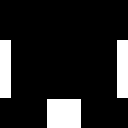
\includegraphics[width=0.31\linewidth]{../outputs/creeper_128.png}
    
\includegraphics[width=0.31\linewidth]{../outputs/skeleton_128.png}
    \caption{Imagenes de proyeccion en Z de los modelos Bunny, creeper-like y skeleton-like voxelizados.}
    \label{fig:voxel-projections}
\end{figure}

\section{Resultados}

\begin{table}[t]
    \centering
    \caption{Resultados locales para resolucion 128, mediana de tres ejecuciones.}
    \begin{tabular}{lrrrrr}
        \toprule
        Modo        & $p$ & $T_p$ (s) & $S(p)$ & $E(p)$ & $O/T_s$ \\
        \midrule
        MPI         & 1   & 0.002703  & 1.000  & 1.000  & 0.000   \\
        MPI         & 2   & 0.001755  & 1.540  & 0.770  & 0.299   \\
        MPI         & 4   & 0.002288  & 1.181  & 0.295  & 2.386   \\
        OMP atomic  & 1   & 0.003745  & 1.000  & 1.000  & 0.000   \\
        OMP atomic  & 2   & 0.002837  & 1.320  & 0.660  & 0.515   \\
        OMP atomic  & 4   & 0.002061  & 1.817  & 0.454  & 1.201   \\
        OMP private & 1   & 0.003016  & 1.000  & 1.000  & 0.000   \\
        OMP private & 2   & 0.002748  & 1.098  & 0.549  & 0.822   \\
        OMP private & 4   & 0.002948  & 1.023  & 0.256  & 2.910   \\
        OMP atomic CUDA (local) & 1 & 0.304685 & --- & --- & ---   \\
        \bottomrule
    \end{tabular}
\end{table}

Para resoluciones $32$ y $64$, los tiempos medidos son muy pequenos y el
overhead domina. En resolucion $128$, MPI obtiene su mejor punto local con
$p=2$. OpenMP atomic mejora hasta $p=4$ en esta malla pequena, mientras que
OpenMP private no supera claramente a las otras variantes porque la reduccion de
grillas privadas es significativa en comparacion con el computo.

\begin{table}[t]
    \centering
    \caption{Resultados MPI sobre Stanford Bunny.}
    \begin{tabular}{rrrrr}
        \toprule
        $r$ & $p$ & $T_p$ (s) & $S(p)$ & $E(p)$ \\
        \midrule
        128 & 1 & 0.012897 & 1.000 & 1.000 \\
        128 & 2 & 0.007408 & 1.741 & 0.871 \\
        128 & 4 & 0.004490 & 2.873 & 0.718 \\
        128 & 8 & 0.005638 & 2.288 & 0.286 \\
        512 & 1 & 0.078667 & 1.000 & 1.000 \\
        512 & 2 & 0.062191 & 1.265 & 0.632 \\
        512 & 4 & 0.085296 & 0.922 & 0.231 \\
        512 & 8 & 0.105886 & 0.743 & 0.093 \\
        \bottomrule
    \end{tabular}
\end{table}

Los resultados con Bunny muestran el mismo patron de strong scaling visto en el
curso: para un problema fijo, el mejor $p$ es finito. En $r=128$, el mayor numero
de triangulos amortiza el overhead de MPI hasta $p=4$. En $r=512$, la reduccion
de la grilla densa y el trafico de memoria dominan despues de $p=2$ en la
ejecucion medida en laptop.

\subsection{Escalabilidad y Comparacion Teorica}

El modelo teorico predice que la parte computacional deberia disminuir
aproximadamente como $C/p$. El speedup experimental sigue esta tendencia solo
mientras el trabajo local de voxelizacion domina sobre los costos de
comunicacion y reduccion. Cuando $p$ aumenta, la reduccion de la grilla empacada
en bits, la sincronizacion y el trafico de memoria se vuelven visibles. Esto
explica por que la mejor configuracion no siempre es el mayor $p$.

\begin{figure}[t]
    \centering
    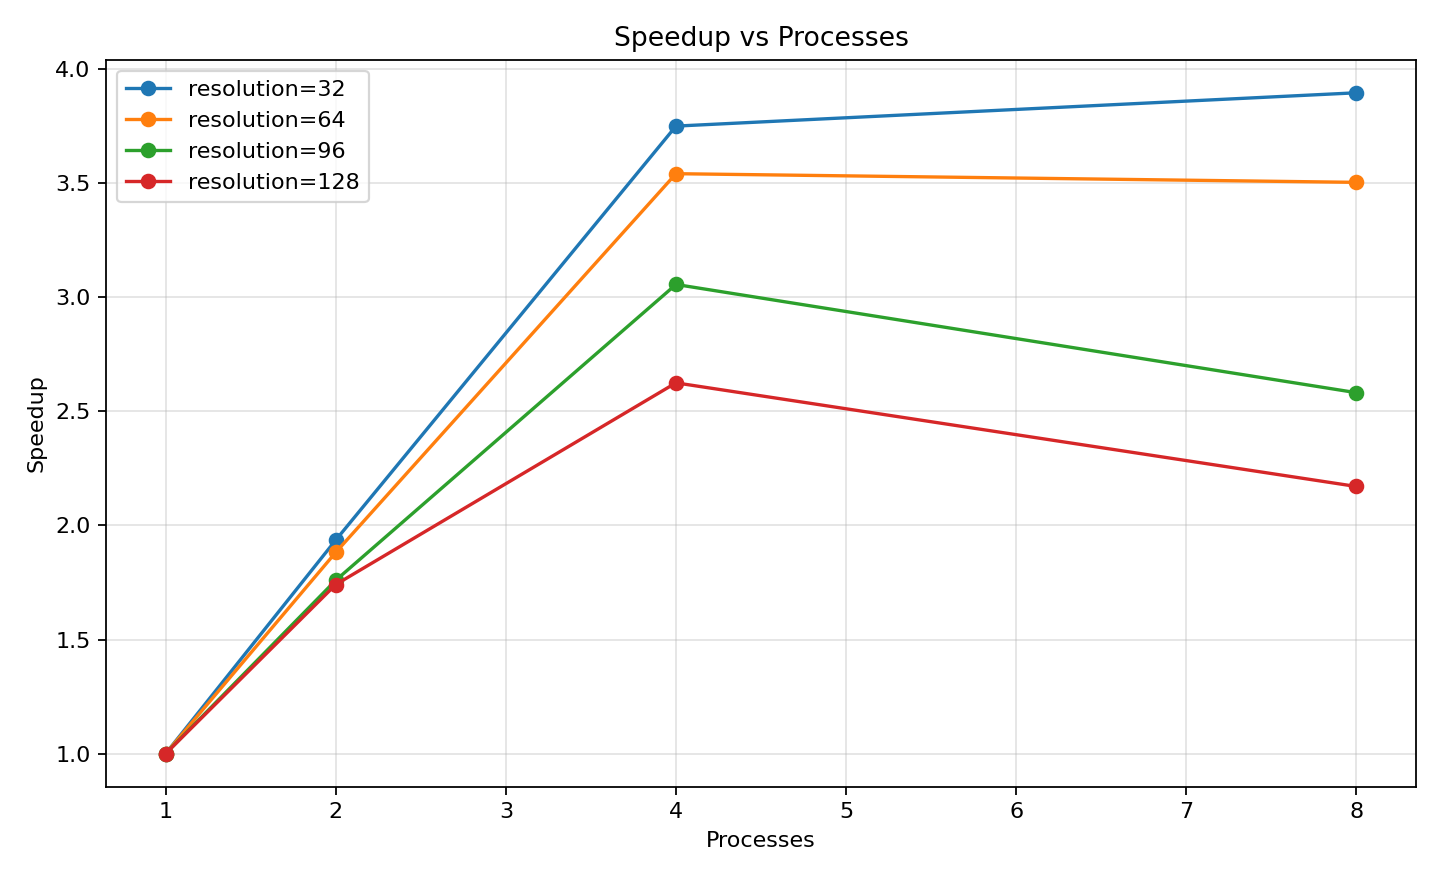
\includegraphics[width=0.48\linewidth]{../results/plots/speedup_vs_processes.png}
    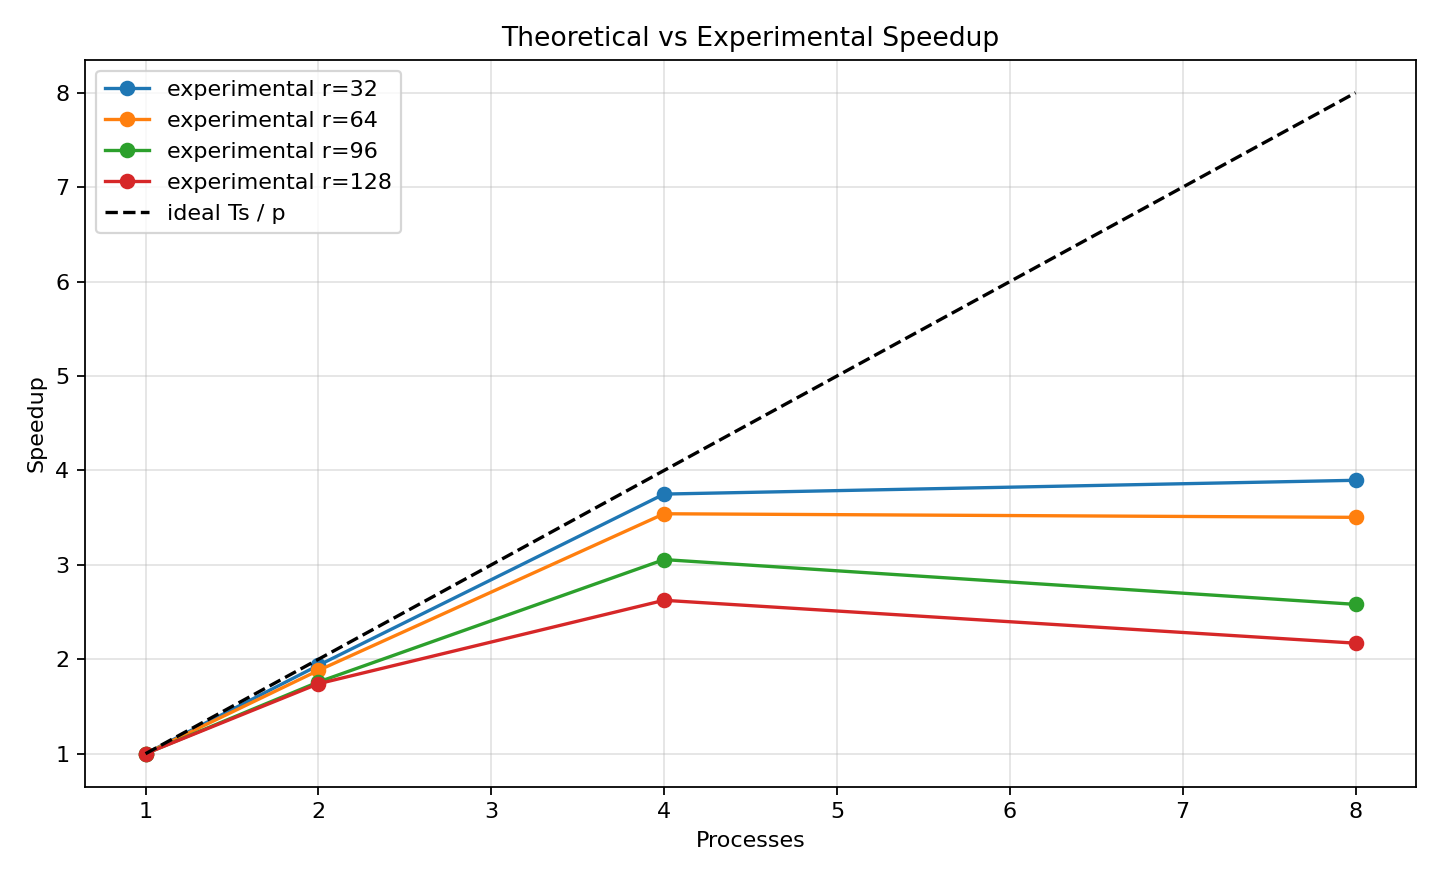
\includegraphics[width=0.48\linewidth]{../results/plots/theoretical_vs_experimental.png}
    \caption{Speedup medido por cantidad de procesos y comparacion contra la tendencia ideal $T_s/p$.}
    \label{fig:speedup-theory}
\end{figure}

La Figura~\ref{fig:speedup-theory} muestra que el speedup medido se acerca a la
curva ideal solo para las primeras cantidades de procesos. Para Stanford Bunny
en $r=128$, el speedup mejora hasta $p=4$ y luego la eficiencia cae en $p=8$.
Esto coincide con el modelo: el termino de computo $C/p$ disminuye, pero
$T_{\text{scatter}}$ y $T_{\text{reduce}}$ permanecen. El termino de reduccion
es especialmente importante porque la grilla tiene $w=\lceil r^3/64\rceil$
palabras.

\begin{figure}[t]
    \centering
    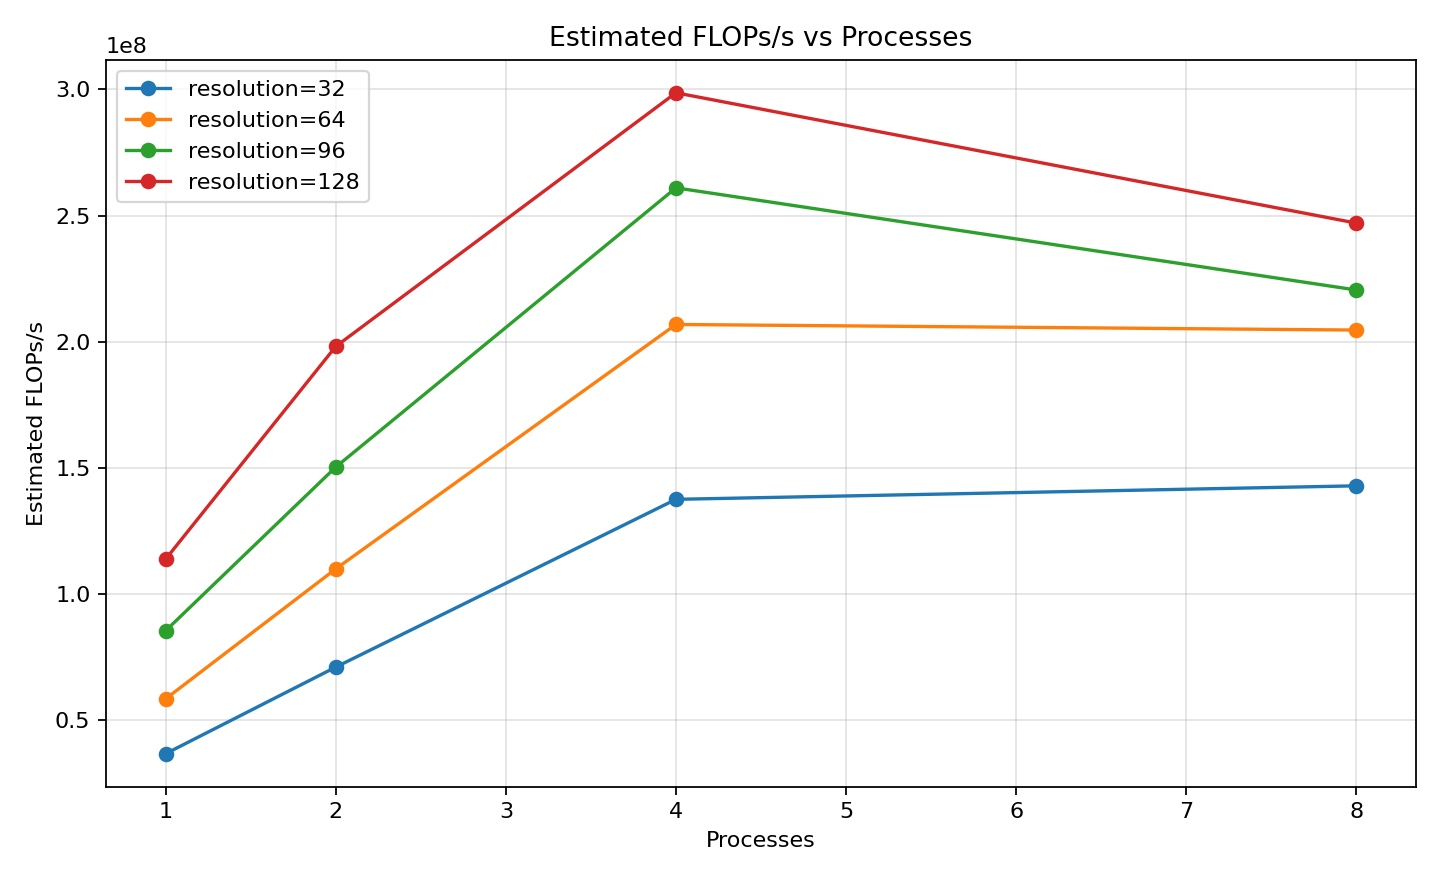
\includegraphics[width=0.48\linewidth]{../results/plots/flops_vs_processes.png}
    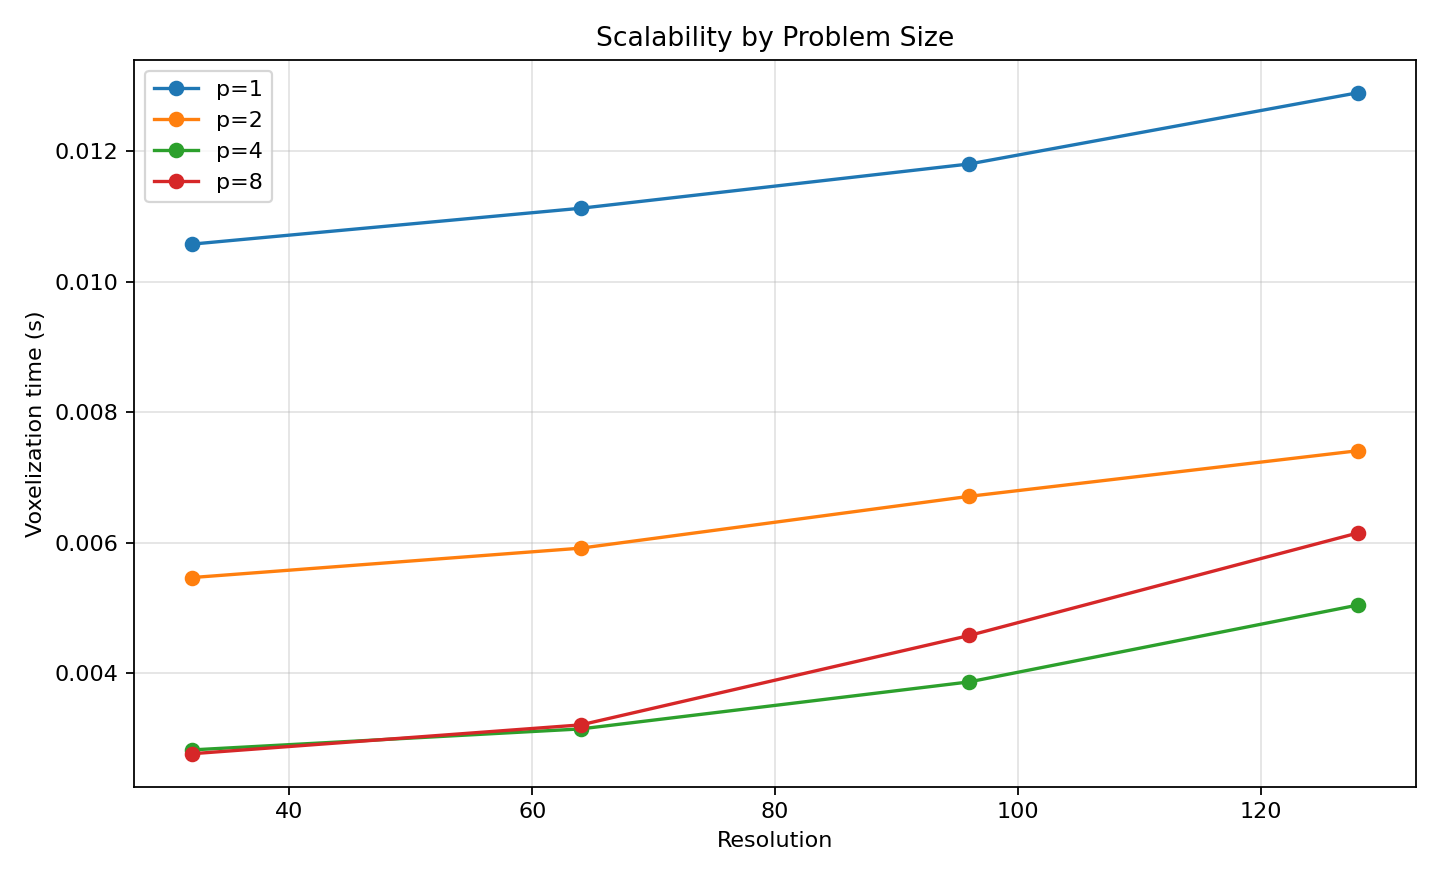
\includegraphics[width=0.48\linewidth]{../results/plots/scalability_by_resolution.png}
    \caption{FLOPs/s estimados y escalabilidad al aumentar la resolucion de grilla.}
    \label{fig:flops-scalability}
\end{figure}

La Figura~\ref{fig:flops-scalability} reporta la curva requerida de FLOPs/s y
el efecto del tamano variable del problema. Aumentar $r$ incrementa la cantidad
de voxels como $r^3$ y tambien incrementa el tamano de la reduccion del bitset.
Por ello, resoluciones mayores exponen mas trabajo, pero tambien mas trafico de
memoria. Los resultados muestran el tradeoff esperado: cantidades moderadas de
procesos amortizan el overhead paralelo, mientras que cantidades altas pueden
perder eficiencia cuando dominan la comunicacion y la reduccion de grilla.

\section{Validacion en Khipu}

El proyecto tambien fue validado en el cluster Khipu de UTEC usando Slurm,
OpenMPI y CMake. El codigo fue ajustado para poder compilar sin Assimp mediante
un pequeno cargador OBJ de respaldo para modelos de benchmark. Se uso un job de
depuracion conservador con hasta cuatro CPUs y resoluciones pequenas. Esta
ejecucion se considera validacion de portabilidad, no un benchmark definitivo,
porque los tiempos medidos estan en el rango de microsegundos a milisegundos y
por eso son sensibles al ruido del scheduler y del entorno.

Se observo un problema operativo: el entorno disponible de OpenMPI no funciono
correctamente con ejecucion directa mediante \texttt{srun} para este programa.
El enfoque estable fue reservar recursos con Slurm y usar \texttt{mpirun} dentro
de la asignacion.

\begin{table}[t]
    \centering
    \caption{Resultados de depuracion GPU en Khipu para el modelo blocky.}
    \begin{tabular}{lrrr}
        \toprule
        Modo & $r$ & $T_p$ (s) & Voxels probados \\
        \midrule
        MPI $p=1$ & 128 & 0.000639 & 277944 \\
        OMP atomic $t=4$ & 128 & 0.002261 & 277944 \\
        CUDA atomic & 128 & 0.311759 & 277944 \\
        MPI $p=1$ & 512 & 0.022754 & 4380856 \\
        OMP atomic $t=4$ & 512 & 0.042784 & 4380856 \\
        CUDA atomic & 512 & 0.410128 & 4380856 \\
        \bottomrule
    \end{tabular}
\end{table}

El prototipo CUDA produjo los mismos conteos de voxels ocupados que las versiones
CPU, pero fue mas lento para los casos pequenos y medianos evaluados. Esto
respalda la decision de no usar este port directo a CUDA como entrega principal.

\section{Discusion}

Los resultados muestran que aumentar $p$ no siempre reduce el tiempo de
ejecucion. En strong scaling, el tamano del problema se mantiene fijo, por lo
que el computo local disminuye aproximadamente como $C/p$, pero los costos de
reduccion, sincronizacion, lanzamiento y memoria no desaparecen. Por ello, el
mejor $p$ no necesariamente es el mayor $p$ disponible.

MPI es defendible como implementacion principal porque representa directamente
memoria distribuida, evita escrituras concurrentes mediante grillas privadas y
expresa la combinacion final como una reduccion OR bit a bit natural. OpenMP es
mas simple en una sola maquina y puede tener menor overhead, pero sus variantes
exponen costos distintos: las grillas privadas consumen memoria y ancho de banda
de reduccion, mientras que las actualizaciones atomicas pueden sufrir contencion.

La principal debilidad del particionamiento por triangulos es el balance de
carga. Si una malla tiene solo unos pocos triangulos grandes, algunos
trabajadores pueden recibir mucho mas trabajo que otros. Un algoritmo basado en
tiles podria asignar regiones disjuntas de voxels a los trabajadores y eliminar
la reduccion OR final, pero una implementacion ingenua por tiles compararia
demasiados triangulos contra demasiados voxels. Su trabajo es
$\Theta(mr^3/p)$ por paso paralelo sin filtrado espacial, mientras que la
implementacion actual basada en triangulos solo visita
$C=\sum_i c_i$ voxels candidatos. Por ejemplo, una malla con $69{,}451$
triangulos en $r=512$ implicaria cerca de $9.3\times10^{12}$ pruebas
triangulo-voxel en el enfoque ingenuo de todos-los-triangulos-por-tile. Los
voxelizadores practicos basados en tiles necesitan estructuras de filtrado
espacial como binning, BVH, octrees o grillas dispersas.

\subsection{Por que CUDA No Fue la Entrega Principal}

CUDA es tecnicamente atractivo, especialmente cuando se dispone de una GPU local,
y el prototipo \texttt{cuda\_atomic} implementado confirma que el proyecto puede
ejecutarse en la GPU Tesla T4 de Khipu. Sin embargo, la limitacion no es solo si
se puede lanzar un kernel. Una version rapida en GPU necesita un mejor layout de
memoria, menos contencion atomica, medicion de transferencias y validacion de
salida contra la implementacion en CPU.

El costo de memoria tambien crece rapidamente para grillas densas. Una grilla
empacada en bits requiere $r^3/8$ bytes, mientras que una grilla de un byte por
voxel requiere $r^3$ bytes. En $r=4096$, la grilla empacada en bits ya necesita
8 GiB, y una grilla de bytes necesita 64 GiB. Si cada bloque o trabajador de GPU
almacena cuatro grillas privadas empacadas antes de reducir, el mismo caso
$r=4096$ necesita 32 GiB, por encima de una GPU local de 12 GiB. Con 12 GiB de
VRAM, el maximo teorico para una grilla densa empacada en bits es
aproximadamente $r=4688$ para una sola grilla, alrededor de $r=2953$ con cuatro
grillas privadas, y cerca de $r=2344$ con ocho grillas privadas, sin contar
triangulos, buffers auxiliares, overhead del runtime de CUDA y reducciones
temporales.

Estos limites se probaron localmente en una NVIDIA GeForce RTX 5070, que tiene
12 GiB de VRAM. El prototipo \texttt{cuda\_atomic} se ejecuto correctamente para
casos hasta $r=2048$, pero fallo para $r=4096$ y resoluciones superiores por
limitaciones de memoria.

Por lo tanto, CUDA es trabajo futuro razonable solo si se acompana de una mejor
estrategia de memoria, como binning por tiles, reducciones a nivel de bloque o
grillas dispersas. Para esta entrega, MPI y OpenMP siguen siendo la comparacion
principal y defendible entre overhead de memoria distribuida y compartida,
mientras que \texttt{cuda\_atomic} se reporta como un prototipo validado pero no
competitivo.

\section{Conclusion}

La implementacion final mantiene MPI como solucion principal, agrega variantes
OpenMP para comparacion e incluye un prototipo CUDA atomico minimo. Los
experimentos confirman que el overhead es central en el analisis: para grillas
pequenas, el paralelismo puede perder frente al overhead, mientras que para
grillas fijas mas grandes algunas configuraciones obtienen speedup. El prototipo
CUDA valida la ejecucion en GPU, pero muestra que un port atomico directo no es
suficiente para estos inputs. Como trabajo futuro se debe reemplazar la
aproximacion por marcado de AABB con una prueba triangulo-caja e implementar
particionamiento GPU por tiles con filtrado espacial.

\section*{Uso de IA}

OpenAI ChatGPT/Codex fue usado como asistente para organizar el informe, revisar
la derivacion de complejidad, comparar los tradeoffs de MPI/OpenMP/CUDA y
preparar documentacion. El codigo, las formulas y las conclusiones fueron
verificados contra la implementacion del repositorio, la documentacion oficial
de MPI/OpenMP/Khipu y las referencias tecnicas siguientes. La IA no fue usada
como fuente primaria para los resultados experimentales.

\begin{thebibliography}{00}
    \bibitem{b1} M. Schwarz and H.-P. Seidel, ``Fast parallel surface and solid voxelization on GPUs,'' \textit{ACM Transactions on Graphics}, vol. 29, no. 6, Article 179, 2010.
    \bibitem{b2} T. Akenine-Moller, ``Fast 3D triangle-box overlap testing,'' \textit{Journal of Graphics Tools}, vol. 6, no. 1, pp. 29--33, 2001.
    \bibitem{b3} I. Foster, \textit{Designing and Building Parallel Programs: Concepts and Tools for Parallel Software Engineering}. Addison-Wesley, 1995.
    \bibitem{b4} Open MPI Project, ``MPI\_Scatterv(3), MPI\_Bcast(3), and MPI\_Reduce(3) manual pages,'' Open MPI Documentation. [Online]. Available: https://www.open-mpi.org/doc/
    \bibitem{b5} OpenMP Architecture Review Board, ``OpenMP API Specification,'' 2024. [Online]. Available: https://www.openmp.org/specifications/
    \bibitem{b6} Open Asset Import Library, ``Assimp: Open Asset Import Library.'' [Online]. Available: https://www.assimp.org/
    \bibitem{b7} UTEC Khipu, ``Khipu documentation.'' [Online]. Available: https://docs.khipu.utec.edu.pe/
    \bibitem{b8} OpenAI, ``ChatGPT/Codex,'' large language model, 2026. [Online]. Available: https://chat.openai.com/
\end{thebibliography}

\end{document}
